% This file was generated with po4a. Translate the source file.
%
\documentclass[10pt,table,dvipsnames,compress]{beamer}
\usepackage[utf8]{inputenc}
\usepackage[T1]{fontenc}
\usepackage{graphicx}
\usepackage{longtable}
\usepackage{wrapfig}
\usepackage{rotating}
\usepackage[normalem]{ulem}
\usepackage{amsmath}
\usepackage{amssymb}
\usepackage{capt-of}
\usepackage{hyperref}
\usetheme{default} \useinnertheme{rounded}
\useoutertheme[subsection=false]{miniframes} \date{} \title{Mapas de riesgo
jurisdiccionales para la asignación de la deforestación}
\title[riskmaps]{Mapas de riesgo jurisdiccionales para la asignación de la
deforestación} \definecolor{darkgreen}{RGB}{34,139,34} \usepackage{float}
\usepackage{lmodern} \usepackage{pgf} \usepackage{color}
\usepackage[english,french]{babel} \definecolor{vertmoyen}{RGB}{51,110,23}
\definecolor{blueFRB}{HTML}{31859c} \usecolortheme[named=blueFRB]{structure}
\usepackage{tabularx} \usepackage{layout} \setlength{\LTleft}{-5cm plus 1
fill} \setlength{\LTright}{-5cm plus 1 fill} \usepackage{booktabs}
\usepackage{arydshln} \newcommand{\logit}{\text{logit}}
\newcommand{\bs}[1]{\boldsymbol{#1}}
\newcommand{\R}{\textnormal{\sffamily\bfseries R}}
\newcommand{\pkg}[1]{{\fontseries{b}\selectfont #1}}
\newcolumntype{C}[1]{>{\centering\arraybackslash}m{#1}}

\setbeamertemplate{footline}[frame number]
\setbeamertemplate{frametitle}{\usebeamerfont{frametitle}\insertframetitle\vphantom{g}
\par \centering 
\includegraphics[width=\textwidth]{figs/Barre_couleur} }
\beamertemplatenavigationsymbolsempty

\newif\ifplacelogo
\logo{\ifplacelogo
\includegraphics[width=0.5\textwidth]{figs/partners_logos}\fi}

\AtBeginSection[]{ \placelogotrue \begin{frame} \frametitle{Contorno}
\begin{columns}[c] \begin{column}{0.5\textwidth}
\tableofcontents[sections=1,currentsection] \vspace{0.5cm}
\tableofcontents[sections=2,currentsection] \end{column}
\begin{column}{0.5\textwidth} \tableofcontents[sections=3,currentsection]
\vspace{0.5cm} \tableofcontents[sections=4,currentsection] \end{column}
\end{columns} \end{frame} \placelogofalse }

\AtBeginSubsection[]{}

\hypersetup{
colorlinks=true, linkcolor=Black, filecolor=Maroon, citecolor=Blue,
urlcolor=Maroon}

\urlstyle{same}

\hypersetup{
 pdfauthor={Ghislain Vieilledent}, pdftitle={Mapas de riesgo jurisdiccionales
para la asignación de la deforestación}, pdfkeywords={}, pdfsubject={},
pdfcreator={Emacs 29.3 (Org mode 9.6.15)}, pdflang={Español}}
\begin{document}



{ \setbeamertemplate{navigation symbols}{} \begin{frame}[plain,
noframenumbering] \begin{center} \small{\textbf{Taller FAO -- Santa Marta
(Colombia), Julio 2024}} \end{center} \vspace{-0.5cm} \titlepage
\vspace{-3cm} \begin{center}

\includegraphics[width=\textwidth]{figs/Barre_couleur} \vspace{0.25cm}
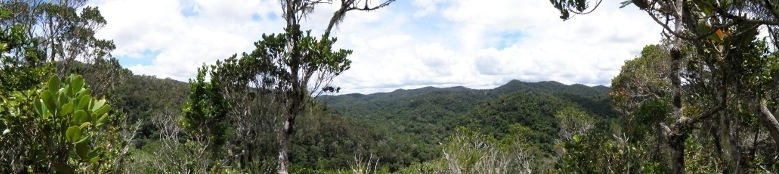
\includegraphics[width=10cm]{figs/Banniere} \small{Ghislain
VIEILLEDENT$^{1}$\hspace{0.25cm}Thomas ARSOUZE$^{1}$\hspace{0.25cm}equipo
FAO$^{2}$} \vspace{0.25cm} {\scriptsize \begin{tabular}{l} $[1]$
\textbf{Cirad} UMR AMAP, $[2]$ \textbf{FAO} Roma y América Latina
\end{tabular} } 
\includegraphics[width=0.8\textwidth]{figs/partners_logos}
\end{center} \end{frame} }


\placelogotrue
\begin{frame}
  \frametitle{Outline}
  \begin{columns}[c]
    \begin{column}{0.5\textwidth} \tableofcontents[sections=1] \vspace{0.5cm}
\tableofcontents[sections=2]
    \end{column}
    \begin{column}{0.5\textwidth} \tableofcontents[sections=3] \vspace{0.5cm}
\tableofcontents[sections=4]
    \end{column}
  \end{columns}
\end{frame}
\placelogofalse

\section{Introducción}
\label{sec:org62b9fb3}

\subsection{Mejorar las metodologías de certificación}
\label{sec:orgabe5ab7}

\begin{frame}[label={sec:org23f7ea1}]{Varias críticas al enfoque basado en proyectos} Se
dirigieron varias críticas a las anteriores metodologías REDD+ para la
certificación de créditos de carbono, acusándolas de sobrevender créditos.

\begin{itemize}
\item \textbf{No adicionalidad}: Las reducciones de emisiones se habrían producido
de todos modos. Niveles de referencia inflados a nivel de proyecto. Los
niveles de referencia jurisdiccionales son razonablemente buenos predictores
de las tendencias futuras.
\item \textbf{Leakage}: Cuanto mayor sea el área cubierta por una iniciativa
REDD+, menor será el riesgo de fuga.
\item \textbf{Reversal}: Las jurisdicciones tienen menos probabilidades que los
proyectos de ver diezmadas sus reservas forestales de carbono por una
perturbación.
\end{itemize}

Frances Seymour (WRI):
\href{https://www.wri.org/insights/insider-4-reasons-why-jurisdictional-approach-redd-crediting-superior-project-based}{Cuatro
razones por las que un enfoque jurisdiccional para la acreditación de REDD+
es superior a un enfoque basado en proyectos}.
\end{frame}

\begin{frame}[label={sec:org792918b}]{Nuevo enfoque jurisdiccional}
\begin{block}{Intensidad de la deforestación}
\begin{itemize}
\item Datos de referencia de la actividad o Nivel de Emisión de Referencia
Forestal a nivel jurisdiccional
\item Cantidad de deforestación.
\item ``Cantidad'' o ``intensidad'' de la deforestación.
\end{itemize}
\end{block}

\begin{block}{Riesgo espacial de deforestación}
\begin{itemize}
\item Mapa del riesgo de deforestación a nivel jurisdiccional.
\item Probabilidad espacial relativa de deforestación.
\item ``Ubicación'' de la deforestación.
\end{itemize}
\end{block}
\end{frame}

\subsection{Asignación de la deforestación a proyectos}
\label{sec:org3bc11bd}

\begin{frame}[label={sec:org9e6b533}]{Mapa de riesgo a nivel jurisdiccional}
\begin{columns}
\begin{column}{0.5\columnwidth}
\begin{block}{Objetivos}
\begin{itemize}
\item Identificación de focos de deforestación.
\item Clasificación de los píxeles forestales en función del riesgo de
deforestación.
\item Un modelo único para toda la jurisdicción (sin discrepancias metodológicas
entre proyectos).
\item Utilice este mapa para asignar la deforestación (estimada para la
jurisdicción) por proyecto.
\end{itemize}
\end{block}
\end{column}

\begin{column}{0.5\columnwidth}
\begin{figure}[htbp]
\centering
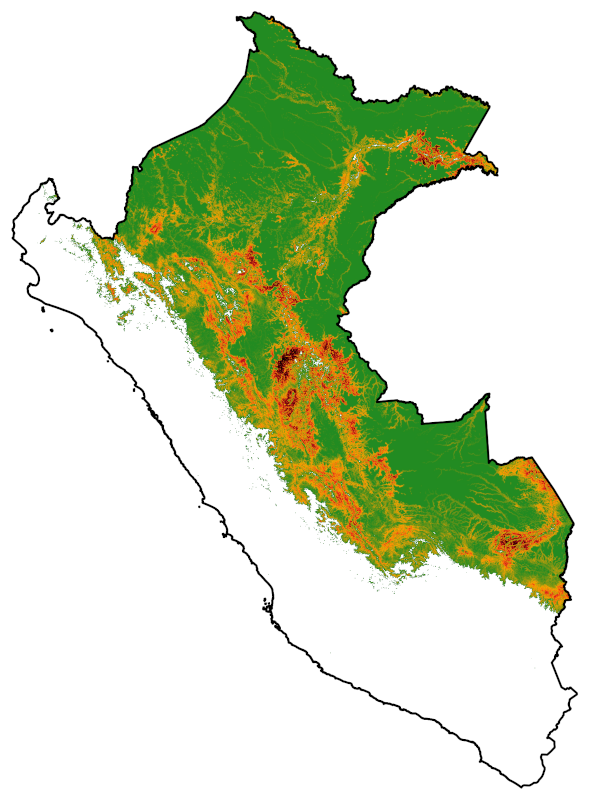
\includegraphics[width=4cm]{figs/prob_PER.png}
\caption{Mapa del riesgo de deforestación en Perou.\newline
\textcolor{darkgreen}{Green} : bajo, \textcolor{red}{Red} /\textbf{Black}:
alto.}
\end{figure}
\end{column}
\end{columns}
\end{frame}

\begin{frame}[label={sec:org7629f10}]{Asignación de la deforestación a proyectos}
\begin{itemize}
\item Mapa de riesgo jurisdiccional: un mapa con clases de riesgo de
deforestación.
\item Obtención de un mapa de densidad de deforestación:\newline Clase de riesgo
de deforestación [1, 2, \ldots{}, \(I\)] \(\rightarrow\) Densidad de
deforestación (ha/año/píxel).
\item Puede utilizarse para asignar la deforestación por proyecto.
\end{itemize}

\begin{figure}[htbp]
\centering
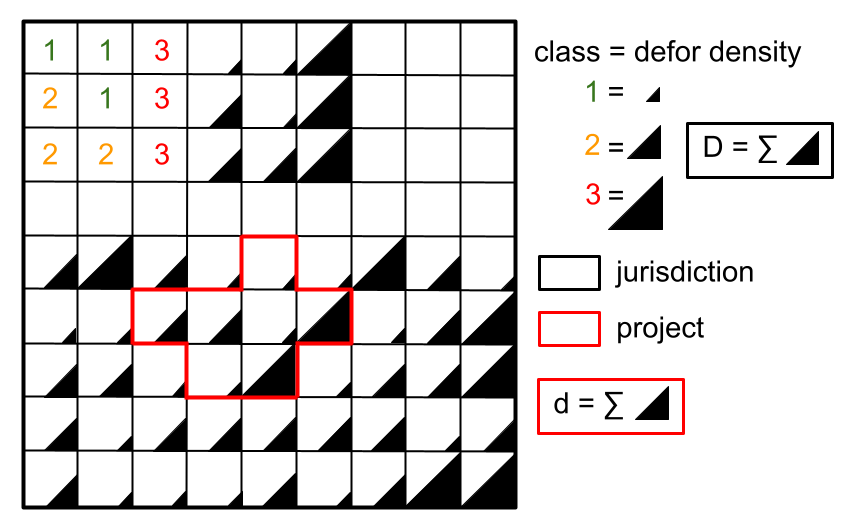
\includegraphics[width=8cm]{figs/get_started/allocation.png}
\caption{Asignación de la deforestación a proyectos dentro de la jurisdicción.}
\end{figure}
\end{frame}

\section{Metodología Verra para la cartografía de riesgos}
\label{sec:orgb558d7e}

\subsection{Herramienta VT0007}
\label{sec:orgdb1d27f}

\begin{frame}[label={sec:orgfbfcecf}]{VT0007 tool}
\begin{itemize}
\item Desarrollado por la Universidad Clark (J. R. Eastman y R. G. Pontius Jr.)
para Verra.
\item \textbf{Aim}: Obtener el mejor mapa de riesgos posible a nivel
jurisdiccional.
\end{itemize}

\begin{block}{Pasos básicos}
\begin{enumerate}
\item Utilizar un modelo de referencia razonablemente bueno para cartografiar el
riesgo de deforestación.
\item Dejar que el usuario proponga mapas alternativos a partir de modelos
alternativos.
\item Fase de validación: comprobar que los modelos alternativos son mejores que
el modelo de referencia.
\item Utilice el mejor mapa alternativo para asignar la deforestación.
\end{enumerate}
\end{block}
\end{frame}

\begin{frame}[label={sec:org224354f}]{Periodos de modelización}
\begin{center}
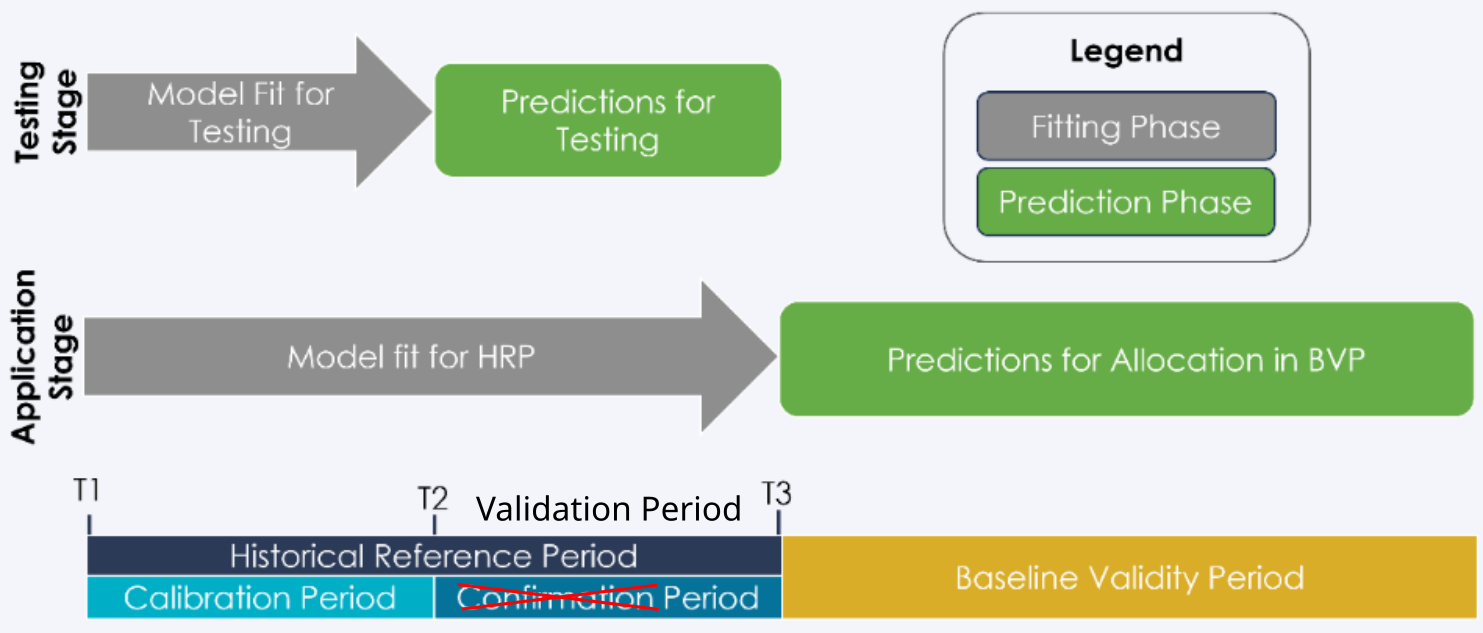
\includegraphics[width=9cm]{figs/get_started/periods.png}
\end{center}

\begin{itemize}
\item Tres fechas: t1, t2, t3.
\item Cuatro periodos: calibración, validación, histórico, (periodo de validez
para el modelo de referencia).
\item Por qué distintos periodos: las predicciones del modelo deben compararse con
\textbf{datos independientes} (periodo de validación).
\item Para hacer previsiones después de t3, queremos utilizar el mayor número de
datos posible (periodo histórico).
\end{itemize}
\end{frame}

\subsection{Modelo de referencia}
\label{sec:orga2b3651}

\begin{frame}[label={sec:org85fc087}]{Modelo de referencia}
\begin{itemize}
\item Modelo de referencia.
\item Un modelo de deforestación razonablemente bueno (mejor que un modelo nulo).
\item Asumiendo una \emph{disminución de la deforestación con la distancia al
borde del bosque} (comúnmente admitido).
\item Y un \emph{modelo diferente entre subjurisdicciones} (variabilidad
regional).
\end{itemize}

\begin{figure}[htbp]
\centering
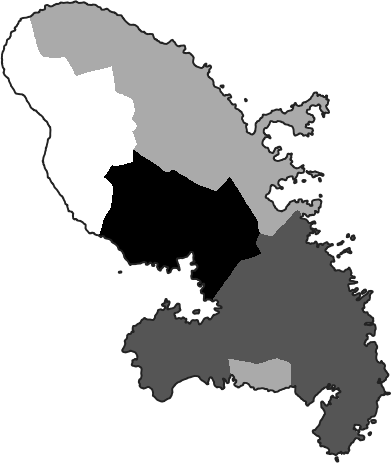
\includegraphics[width=3.5cm]{figs/subj.png}
\caption{Subjurisdicciones en Martinica (MTQ)}
\end{figure}
\end{frame}

\begin{frame}[label={sec:orgb63524a}]{Umbral de distancia}
\begin{itemize}
\item Identifique la distancia al borde del bosque por debajo de la cual se
produce el \textbf{99,5\%} de la deforestación.
\item Utilice esta distancia para definir la primera clase de riesgo (clase 1).
\end{itemize}

\begin{center}
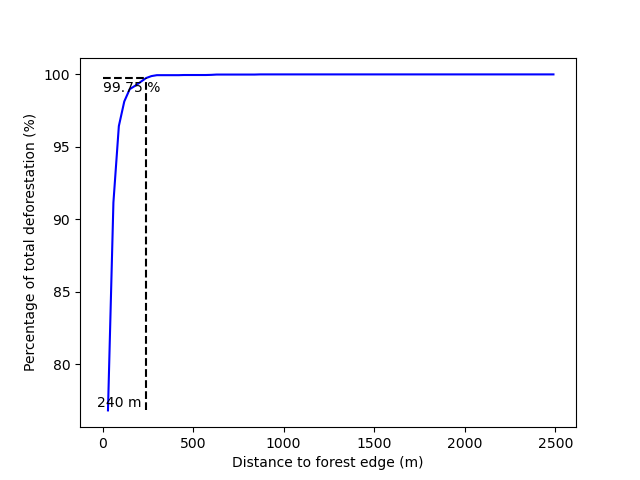
\includegraphics[width=8cm]{figs/get_started/perc_dist.png}
\end{center}
\end{frame}

\begin{frame}[label={sec:org3cf8455}]{De la distancia a la clase de riesgo}
\begin{itemize}
\item Las distancias por debajo del umbral se transforman en clases de riesgo de
deforestación.
\item Para ello se utiliza una serie geométrica que garantiza que las clases
tengan un rango más amplio para distancias mayores.
\item Definimos 29 clases de riesgo adicionales, de la 2 a la 30 (la clase 1 ya
está definida).
\end{itemize}

\begin{center}
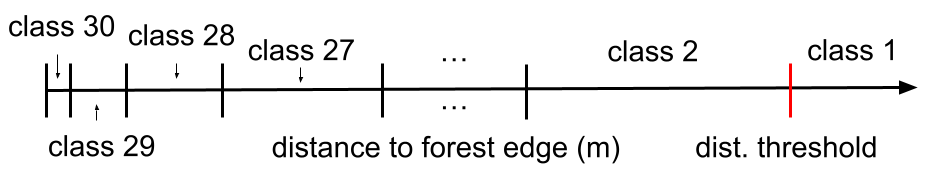
\includegraphics[width=10cm]{figs/dist_class.png}
\end{center}
\end{frame}

\begin{frame}[label={sec:org4b8af87}]{Clases utilizando las subjurisdicciones}
\begin{itemize}
\item Cada subjurisdicción recibe un número del 1 al (potencialmente) 999.
\item Combinamos las clases derivadas de la distancia con las subjurisdicciones de
la siguiente manera: \(\textbf{DD}\text{SSS}\), siendo \textbf{DD} la clase
de distancia y SSS el número de subjurisdicción.
\item Obtenemos clases que van desde 01001 hasta potencialmente 30999 si hay 999
subjurisdicciones.
\item Así, para 10 subjurisdicciones, obtenemos \textasciitilde{}300 clases (pero
pueden faltar algunas clases de distancia).
\end{itemize}
\end{frame}

\begin{frame}[label={sec:org70d692a}]{Clases utilizando las subjurisdicciones}
\begin{itemize}
\item Siguiendo estos pasos, obtenemos un mapa a nivel jurisdiccional en el que
cada píxel de bosque pertenece a una clase determinada de riesgo de
deforestación.
\item Área en verde oscuro: clases \(\mathbf{1}\text{SSS}\), más allá del umbral
de deforestación.
\end{itemize}

\begin{center}
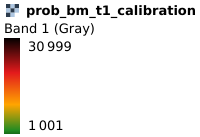
\includegraphics[width=3cm]{figs/prob_bm_t1_legend.png}  
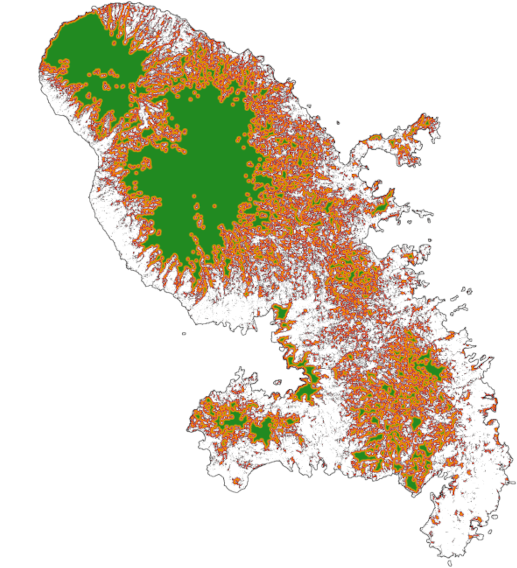
\includegraphics[width=5cm]{figs/prob_bm_t1.png}
\end{center}
\end{frame}

\begin{frame}[label={sec:orgcbb7733}]{Densidad de deforestación}
\begin{itemize}
\item Cada clase \(i\) tiene asociada una \textbf{probabilidad de deforestación}:
\(\theta_{m,i} = d_{i} / n_{i}\) (sin unidades), siendo \(d_{i}\) el número
de píxeles deforestados durante el periodo, y \(n_{i}\) el número de píxeles
forestales al principio del periodo.
\item \textbf{Ajuste de la cantidad \(\rho\)}: \(\theta_{a,i} = \rho
\theta_{m,i}\), de modo que la deforestación total prevista = deforestación
observada (o esperada). Para el modelo de referencia para la calibración y
los periodos históricos, \(\rho=1\).
\item \textbf{Densidad de deforestación (en ha/año por píxel)} calculada como
\(\delta_{i} = \theta_{a,i} \times A / T\). \(A\): superficie del píxel (en
ha), \(T\): intervalo de tiempo del periodo (en años).
\item La densidad de deforestación se utiliza para predecir la cantidad de
deforestación de cada píxel perteneciente a una determinada clase de riesgo
de deforestación.
\end{itemize}
\end{frame}

\begin{frame}[label={sec:orgf2b4ad4}]{Densidad de deforestación}
\begin{table}[htbp]
\caption{\label{tab:org09a753e}Tasas de deforestación para cada clase de riesgo de deforestación (cifras
truncadas a tres dígitos decimales).}
\small
\begin{tabular}{rrrrrrrr}
\toprule cat & \(n_i\) & \(d_i\) & \(\theta_{m,i}\) & \(\theta_{a,i}\) & \(T\) & \(A\) & \(\delta_{i}\)\\[0pt] \midrule 1001 & 33433 & 0 & 0.0 & 0.0 & 10 & 0.09 & 0.0\\[0pt] 1002 & 12965 & 0 & 0.0 & 0.0 & 10 & 0.09 & 0.0\\[0pt] 1003 & 91686 & 19 & 2.072e-04 & 2.072e-04 & 10 & 0.09 & 1.865e-06\\[0pt] 1004 & 82279 & 5 & 6.076e-05 & 6.076e-05 & 10 & 0.09 & 5.469e-07\\[0pt] 2001 & 1373 & 0 & 0.0 & 0.0 & 10 & 0.09 & 0.0\\[0pt] \bottomrule
\end{tabular}
\end{table}

\textbf{Densidad de deforestación (en ha/año por píxel)} calculada como
\(\delta_{i} = \theta_{a,i} \times A / T\)
\end{frame}

\begin{frame}[label={sec:org8465960}]{Densidad de deforestación} La densidad de
deforestación puede utilizarse para asignar la deforestación a proyectos
dentro de una jurisdicción.

\begin{figure}[htbp]
\centering
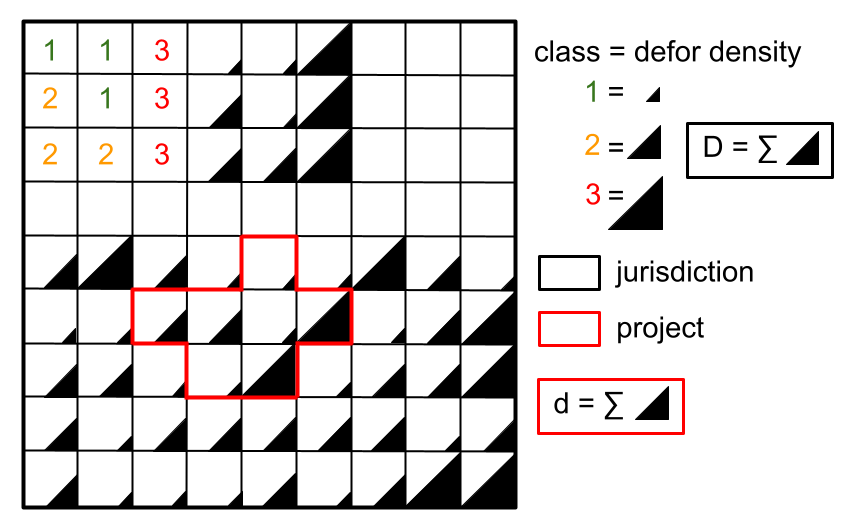
\includegraphics[width=8cm]{figs/get_started/allocation.png}
\caption{Asignación de la deforestación a proyectos dentro de la jurisdicción.}
\end{figure}
\end{frame}

\subsection{Modelos alternativos y validación}
\label{sec:org8cdbf76}

\begin{frame}[label={sec:org84a06d6}]{Modelos alternativos}
\begin{itemize}
\item Los mapas alternativos utilizando modelos alternativos deben compararse con
el modelo de referencia.
\item El modelo alternativo puede ser de diferentes formas: modelo de
geoprocesamiento (ventana móvil), modelo estadístico (iCAR, GLM, RF).
\item Por ejemplo, Clark Labs propone el modelo estadístico MLP (Multi-Layer
Perceptron) en el módulo Land Change Modeller del software
\href{https://clarklabs.org/terrset/}{TerrSet}.
\end{itemize}
\end{frame}

\begin{frame}[label={sec:org2f962a4}]{Modelos alternativos}
\begin{itemize}
\item Debe facilitarse un mapa de riesgo con las densidades de deforestación
derivadas del modelo alternativo.
\end{itemize}

\begin{figure}[htbp]
\centering
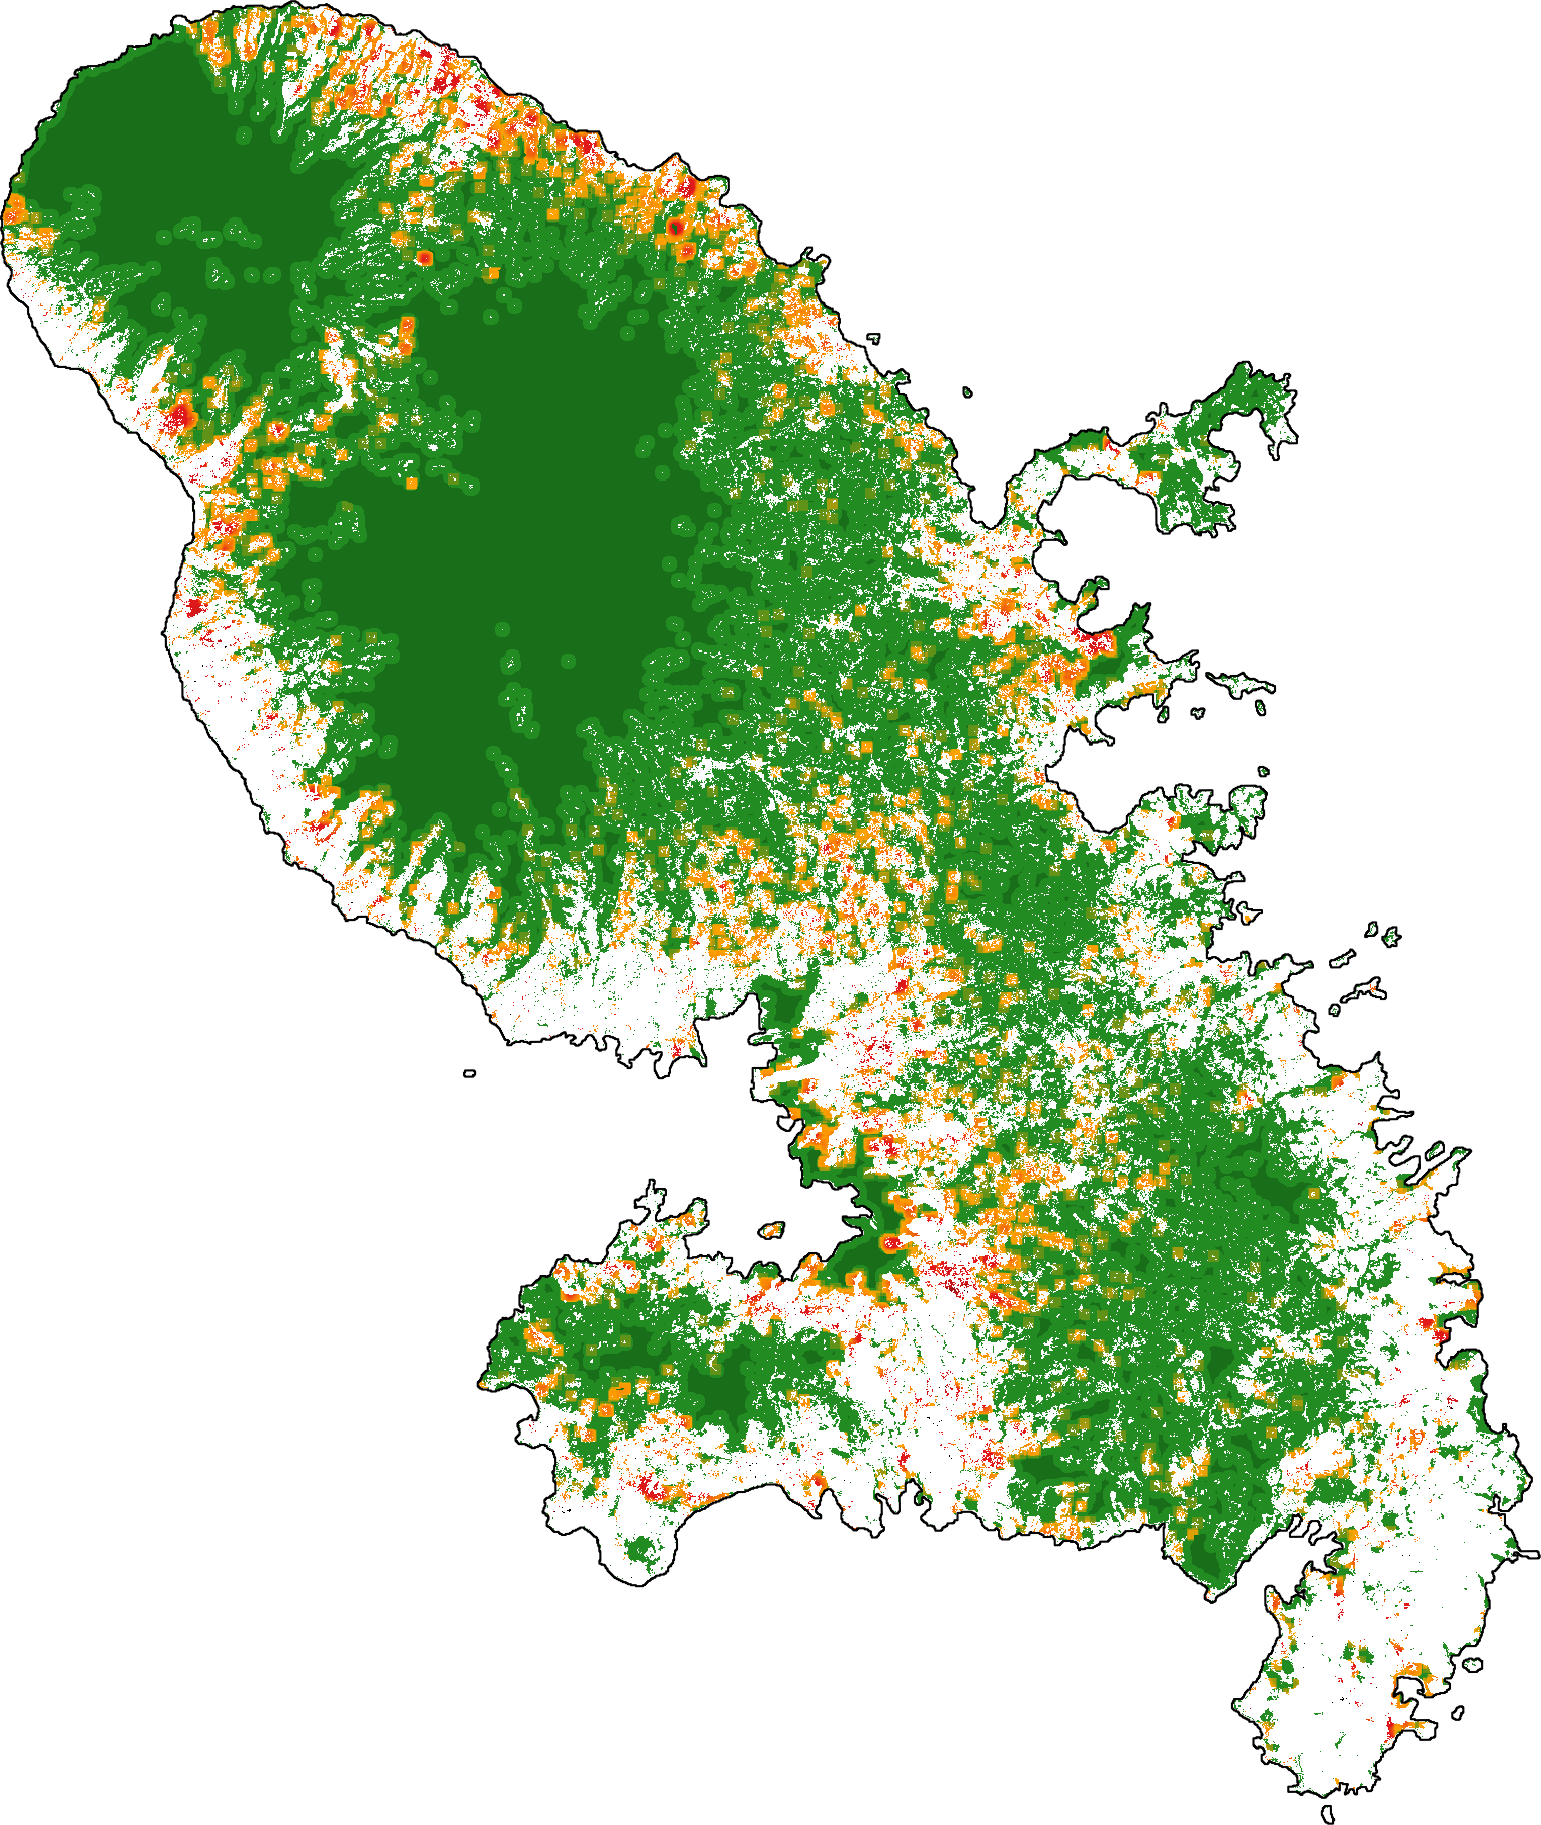
\includegraphics[width=4.5cm]{figs/prob_mw_11_t1.png}
\caption{Mapa de riesgo obtenido con un modelo de ventana móvil.}
\end{figure}
\end{frame}

\begin{frame}[label={sec:orgaf08b6a}]{Procedimiento de validación}
\begin{itemize}
\item Comparación de la deforestación prevista frente a la observada (en ha) en
una cuadrícula gruesa.
\item Durante un periodo de tiempo determinado.
\end{itemize}

\begin{figure}[htbp]
\centering
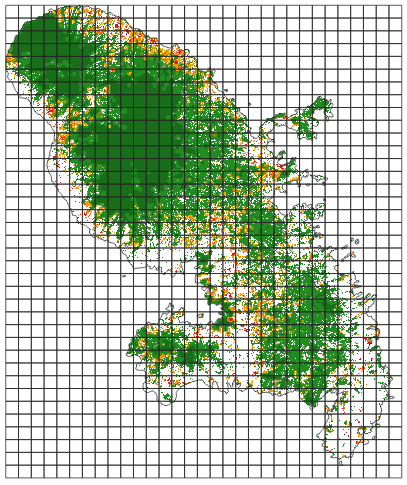
\includegraphics[width=4.5cm]{figs/grid.png}
\caption{Cuadrícula gruesa que cubre el área de interés.}
\end{figure}
\end{frame}

\begin{frame}[label={sec:org1e5fa33}]{Procedimiento de validación}
\begin{itemize}
\item Comparación entre la deforestación prevista y la observada.
\item Índices de rendimiento: \(R^2\), y mediana del error absoluto (MedAE).
\end{itemize}

\begin{center}
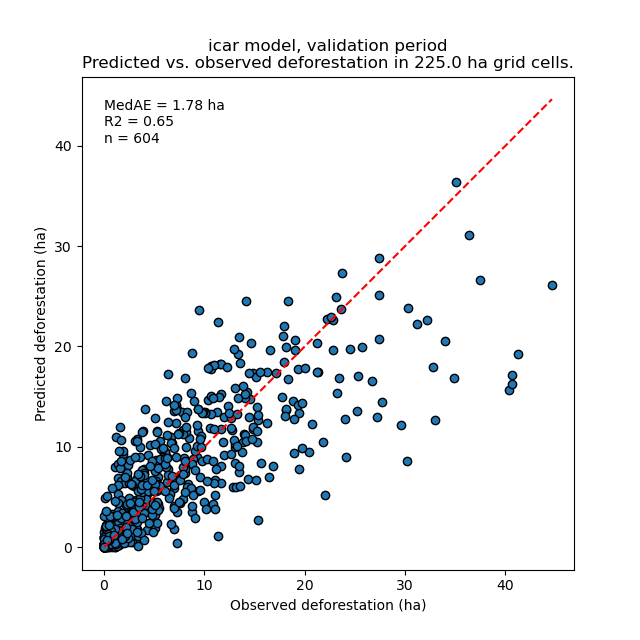
\includegraphics[width=6.5cm]{figs/get_started/pred_obs_icar_validation_50.png}
\end{center}
\end{frame}

\begin{frame}[label={sec:org0e055a9}]{Procedimiento de validación}
\begin{itemize}
\item Se calculan índices de rendimiento para cada modelo.
\item Se selecciona el modelo con mayor \(R^2\) y menor MedAE.
\end{itemize}

\begin{table}[htbp]
\caption{\label{tab:orga96bff6}Índices de rendimiento.}
\small
\begin{tabular}{rllrrrr}
\toprule ncell & periodo & modelo & MedAE & R2 & RMSE & wRMSE\\[0pt] \midrule 604 & validación & bm & 2.71 & 0.43 & 6.08 & 6.22\\[0pt] 604 & validación & icar & 1.78 & 0.65 & 4.79 & 4.59\\[0pt] 604 & validación & glm & 2.39 & 0.38 & 6.39 & 6.52\\[0pt] 604 & validación & rf & 2.09 & 0.50 & 5.69 & 5.74\\[0pt] 604 & validación & mw\_11 & 2.34 & 0.56 & 7.66 & 6.83\\[0pt] 604 & validación & mw\_21 & 2.51 & 0.56 & 7.54 & 6.66\\[0pt] \bottomrule
\end{tabular}
\end{table}
\end{frame}

\begin{frame}[label={sec:orgfc9200d}]{Procedimiento de validación}
\begin{center}
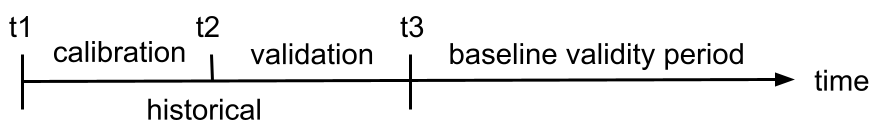
\includegraphics[width=.9\linewidth]{figs/periods.png}
\label{org9c58444}
\end{center}

\begin{itemize}
\item Podemos comparar la deforestación prevista frente a la observada para tres
periodos de tiempo: \textbf{calibración}, \textbf{validación} y
\textbf{periodo histórico}.
\item Estimar el rendimiento del modelo para predecir la deforestación en el
futuro: \textbf{deforestación prevista frente a la observada} para el
\textbf{periodo de validación} con un modelo ajustado durante el
\textbf{periodo de calibración}.
\item De este modo, utilizamos \textbf{observaciones independientes} de la
deforestación para la validación del modelo (la deforestación observada
durante el periodo de validación no se ha utilizado para calibrar el
modelo).
\item Metodología de Verra: el modelo alternativo debe ser mejor tanto para el
periodo de calibración como para el de validación.
\end{itemize}
\end{frame}

\section{Programa informático de cartografía del riesgo de deforestación}
\label{sec:org9fa4114}

\subsection{Software Verra/Clark Labs}
\label{sec:orge59843f}

\begin{frame}[label={sec:orgd16808a}]{Software Verra/Clark Labs}
\begin{center}
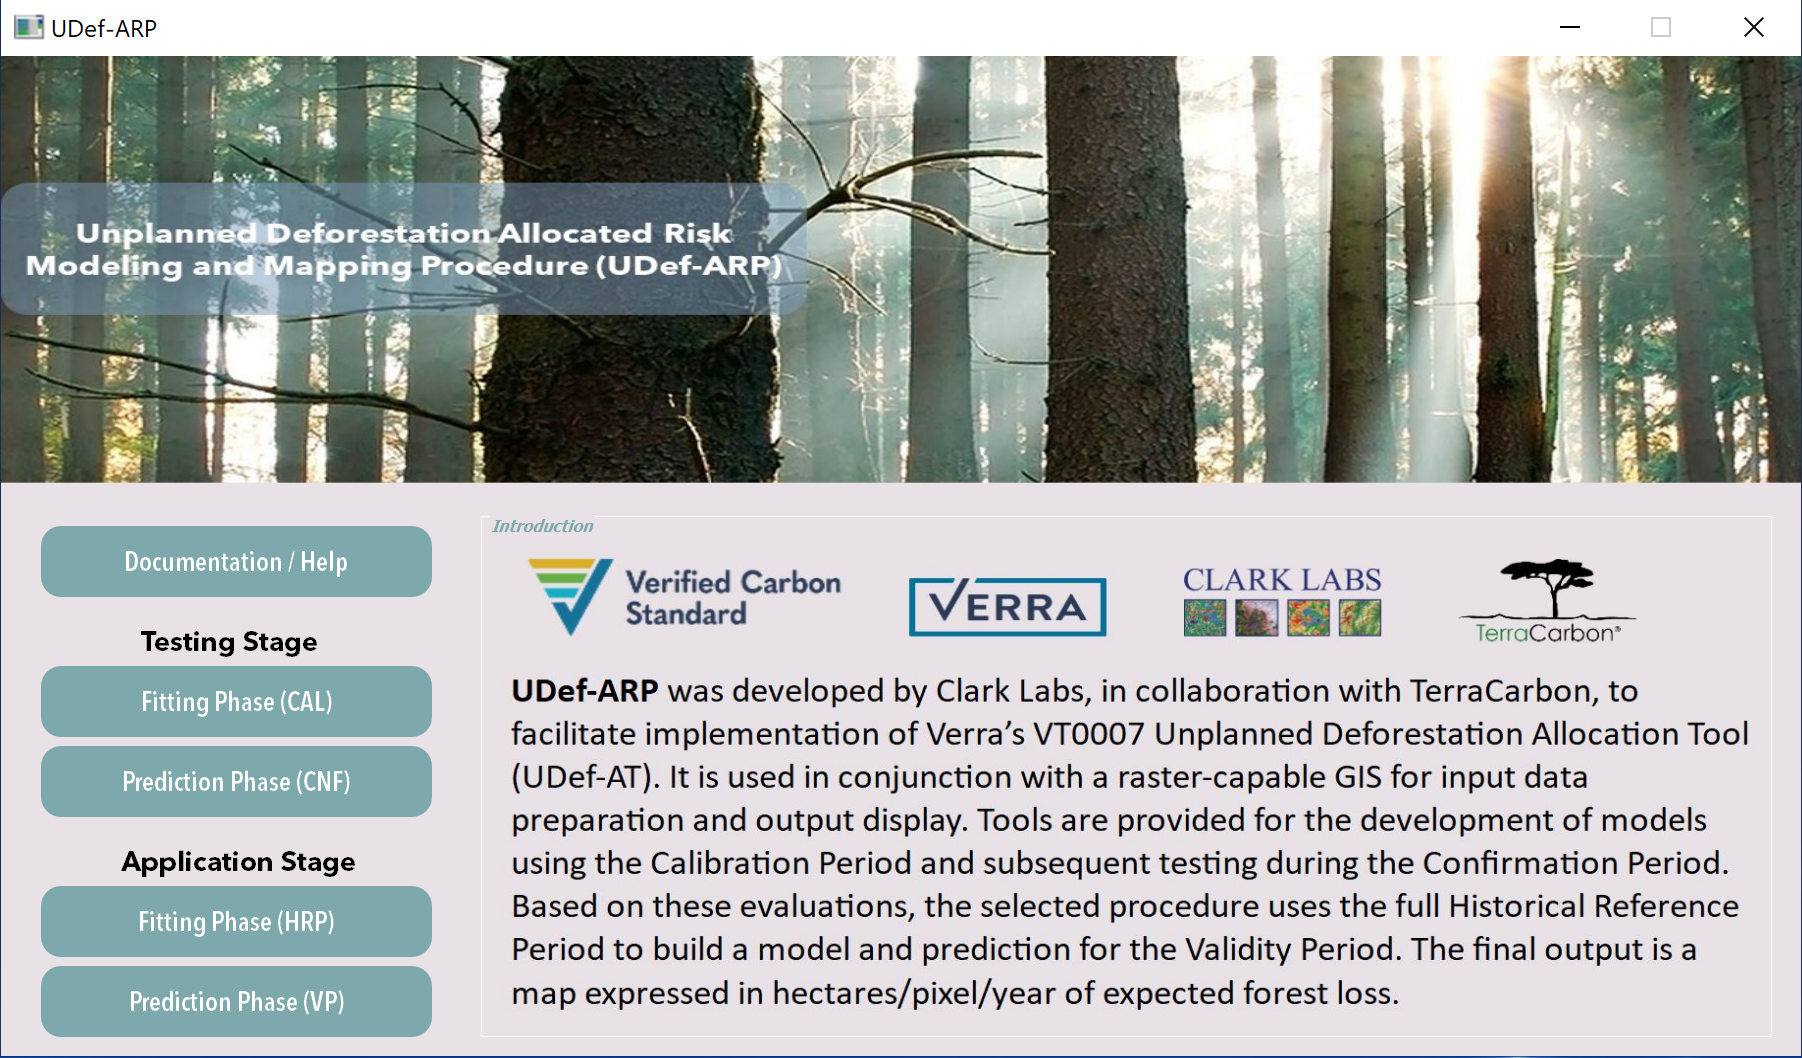
\includegraphics[width=9cm]{figs/verra_tool.png}
\end{center}

\centering Aplicación independiente: \url{https://github.com/ClarkCGA/UDef-ARP} \\[0pt]
\centering Plugin QGIS: \url{https://github.com/ClarkCGA/UDef-ARP-Plugin}
\end{frame}

\begin{frame}[label={sec:org4e71f43}]{Software Verra/Clark Labs}
\begin{center}
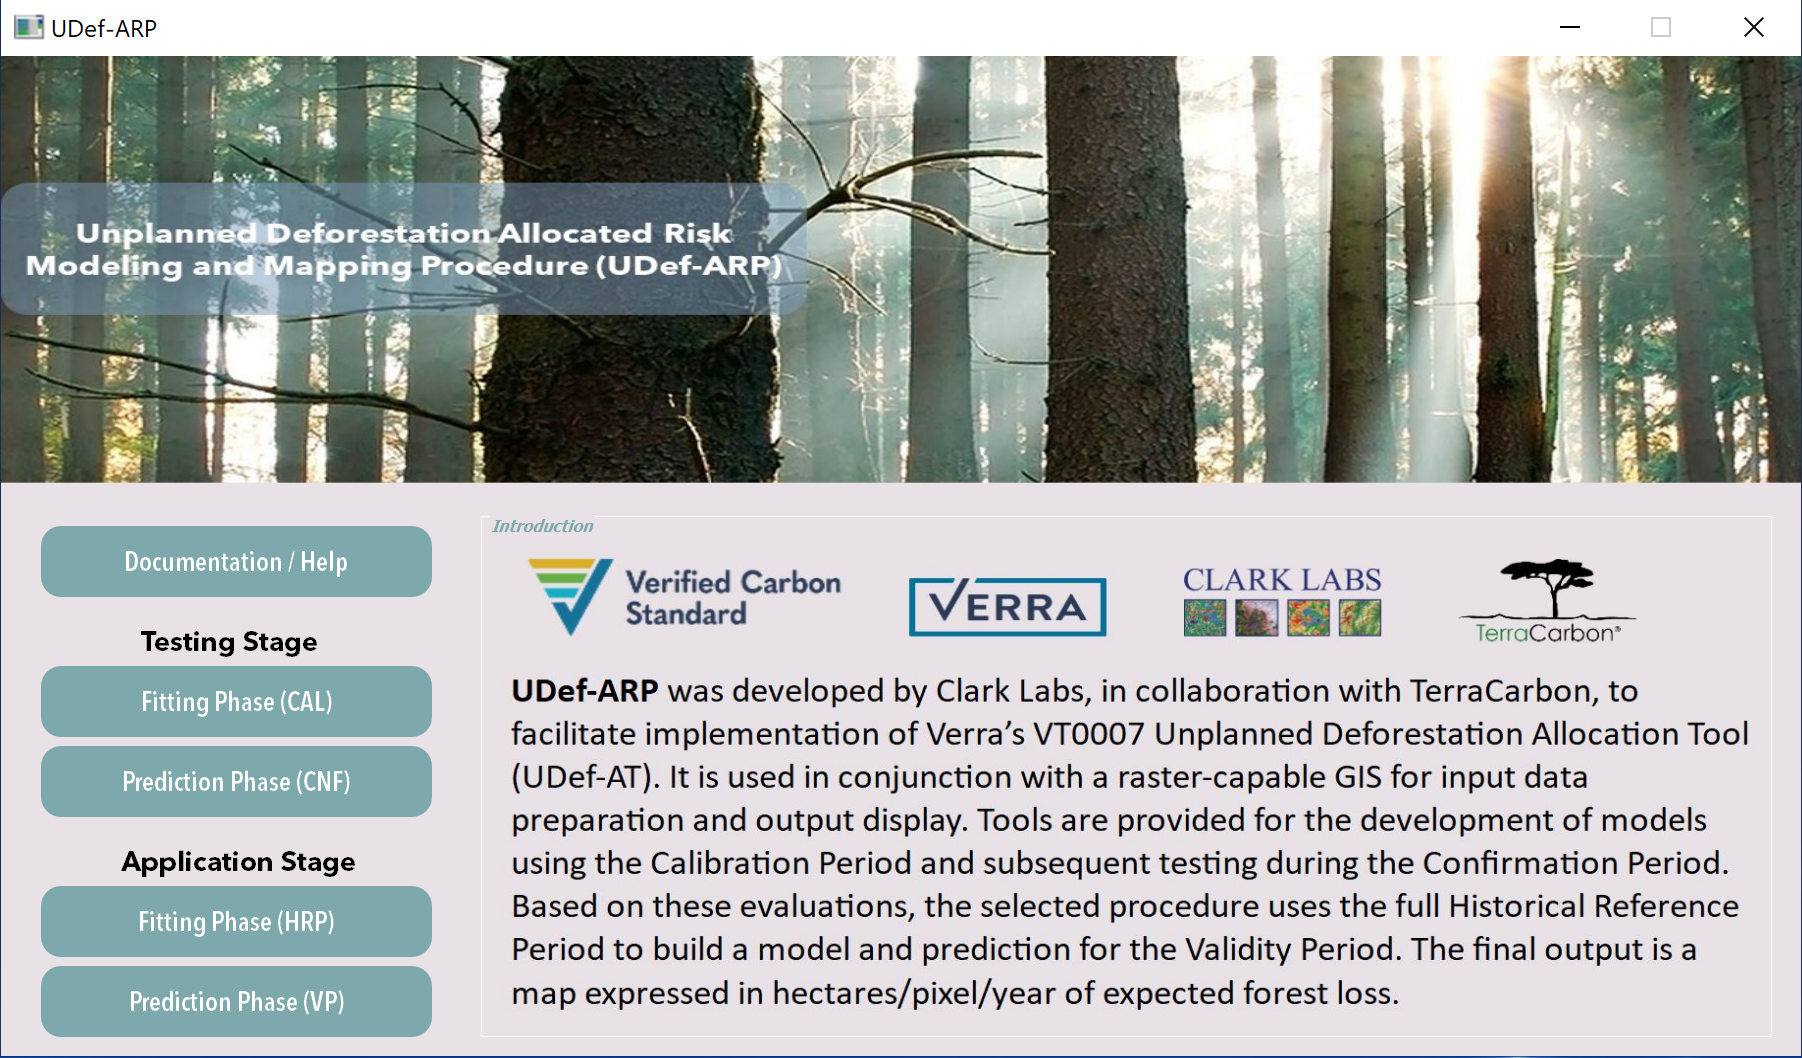
\includegraphics[width=6cm]{figs/verra_tool.png}
\end{center}

\begin{itemize}
\item El usuario debe proporcionar rásters: cambio de la cubierta forestal,
distancia al borde del bosque en varias fechas, fronteras
subjurisdiccionales, mapas de riesgo alternativo en varias fechas.
\item A partir de estos datos, la UDef-ARP proporciona la base:
\begin{itemize}
\item para desarrollar un modelo de referencia.
\item para comparar el modelo de referencia y los modelos alternativos.
\end{itemize}
\end{itemize}
\end{frame}

\begin{frame}[label={sec:orgab23372}]{Limitaciones}
\begin{itemize}
\item No hay ninguna herramienta que ayude a preparar los datos.
\item No hay herramienta que ayude a desarrollar los \textbf{modelos
alternativos}.
\item Sólo Windows (de momento).
\item Se requiere un ordenador con mucha RAM para una jurisdicción grande: todos
los rásters se almacenan en RAM durante el procesamiento. Por lo tanto, las
jurisdicciones de gran tamaño \textbf{requieren importantes asignaciones de
RAM} (por ejemplo, 64Gb).
\item Uso de data de tipo Float para mapas de riesgo con densidad de deforestación
(ha/pixel/año): \textbf{gran espacio en disco}.
\item Documentación sólo en inglés, \textbf{no hay traducciones disponibles}.
\item Herramienta reciente, algunos comentarios de los usuarios (por ejemplo,
Fronterra):
\href{https://www.linkedin.com/posts/fron-terra\_forest-carbon-climatechange-activity-7179166090042732544-YnAK?utm\_source=share\&utm\_medium=member\_desktop}{Post
1},
\href{https://www.linkedin.com/posts/fron-terra\_forest-carbon-climatechange-activity-7179721587267371008-PRXr?utm\_source=share\&utm\_medium=member\_desktop}{Post
2},
\href{https://www.linkedin.com/posts/fron-terra\_carbon-climatechange-verra-activity-7180971577746862080-rolc?utm\_source=share\&utm\_medium=member\_desktop}{Post
3}.
\end{itemize}
\end{frame}

\subsection{Programas informáticos existentes para modelos alternativos}
\label{sec:orgda91c23}

\begin{frame}[label={sec:org3572bfb}]{Software existente para modelos alternativos}
\begin{itemize}
\item \href{https://csr.ufmg.br/dinamica/}{Dinamica EGO}: Universidade Federal de
Minas Gerais, Brazil.
\item \href{https://clarklabs.org/terrset/land-change-modeler/}{Land Change
Modeler}: Clark Labs, Clark University, Worcester, USA.
\item \href{https://www.environmentalgeography.nl/site/data-models/data/clue-model/}{CLUE}:
Institute for Environmental Studies, Vrije Universiteit, Amsterdam,
Netherlands .
\end{itemize}

\vspace{0.25cm}

\textbf{Grandes programas} con muchas aplicaciones. Muchos estudios
científicos, publicados en un gran número de artículos científicos, han
utilizado estos programas.
\end{frame}

\subsection{Limitaciones}
\label{sec:org4838a92}

\begin{frame}[label={sec:org9bf2005}]{Limitaciones}
\begin{itemize}
\item No todos son de código abierto (por ejemplo, Dinamica EGO y LCM):
\textbf{transparencia}.
\item No todos son gratuitos (por ejemplo, LCM): pero hay descuentos para
estudiantes y países en desarrollo.
\item No todos permiten scripts (por ejemplo, LCM, CLUE):
\textbf{reproducibility}.
\item Puede que no funcione con rásters de alta resolución (<= 30 m) en
jurisdicciones grandes (escala de país).
\item Número limitado de modelos estadísticos para modelizar el cambio de uso del
suelo: precisión limitada y ajuste excesivo.
\end{itemize}

\vspace{0.25cm}

Ver \textbf{Vieilledent et al.} 2021, \emph{JOSS}, doi:
\href{https://doi.org/10.21105/joss.02975}{10.21105/joss.02975} para más
detalles.
\end{frame}

\begin{frame}[label={sec:org341817c}]{Limitaciones}
\begin{itemize}
\item La metodología de Verra incluye \textbf{varios pasos} (calibración,
validación, previsión), que deben \textbf{repetirse} (modelo, periodo).
\item Debe ser posible seguir la metodología de Verra con uno de estos programas
(dados algunos requisitos, como un ordenador con mucha RAM).
\item Pero exigiría mucho trabajo al usuario adaptar el uso del programa a la
metodología de Verra (por ejemplo, paso de validación con cuadricula
gruesa).

\item \textbf{Note}: en la documentación de UDef-ARP, Clark Labs indica que tiene
previsto ofrecer próximamente una utilidad para facilitar la creación de
mapas de vulnerabilidad para modelos alternativos.
\end{itemize}
\end{frame}

\section{Conclusión}
\label{sec:org943fe8a}

\subsection{Una metodología no tan sencilla}
\label{sec:orgfd50e8c}

\begin{frame}[label={sec:org4dba697}]{Resumen}
\begin{itemize}
\item Necesitamos un \textbf{mapa del riesgo de deforestación} a \textbf{nivel
jurisdiccional}.
\item Riesgo de deforestación: \textbf{densidad de deforestación} en ha/pixel/año.
\item Este mapa debería ser mejor que el mapa derivado del modelo de referencia.
\item El mejor mapa se utilizará para \textbf{asignar la deforestación} a
proyectos dentro de la jurisdicción.
\end{itemize}
\end{frame}

\begin{frame}[label={sec:orgfa6a091}]{Una metodología no tan sencilla}
\begin{itemize}
\item El mapa de riesgos debe obtenerse siguiendo la metodología Verra/Clark Labs.
\item La metodología se desarrolló pensando en la simplicidad.
\item Pero la modelización de la deforestación es intrínsecamente complicada y la
comparación y validación de modelos requiere un número mínimo de pasos.
\item Esto dificulta el desarrollo de un modelo alternativo mejor que el modelo de
referencia utilizando las herramientas existentes.
\end{itemize}
\end{frame}

\subsection{Necesidad de una herramienta integradora: deforisk plugin}
\label{sec:org7378434}

\begin{frame}[label={sec:org7881967},fragile]{Necesidad de una herramienta integradora:
el plugin QGIS deforisk}
 \begin{itemize}
\item Se necesita una utilidad que facilite la creación de mapas de riesgo para
modelos alternativos.
\item Especificidades:
\begin{itemize}
\item \textbf{Integrative}: todas las etapas de la metodología Verra (modelo de
referencia, modelos alternativos, validación, asignación).
\item \textbf{Precisión}: alta precisión para prever la deforestación.
\item \textbf{Fácil de usar}: interfaz sencilla con documentación.
\item \textbf{Transparente y reproducible}: utilizando software de código abierto
(importante para la certificación de créditos de carbono/biodiversidad).
\end{itemize}
\end{itemize}

\begin{columns}
\begin{column}{0.8\columnwidth}
\begin{itemize}
\item El Cirad y la FAO han trabajado en el desarrollo del plugin
\texttt{deforisk} de QGIS para cumplir estos objetivos:
\url{https://ecology.ghislainv.fr/deforisk-qgis-plugin/es}
\end{itemize}
\end{column}

\begin{column}{0.2\columnwidth}
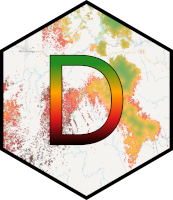
\includegraphics[width=1.5cm]{figs/logo-deforisk.png}
\end{column}
\end{columns}
\end{frame}


{ \usebackgroundtemplate{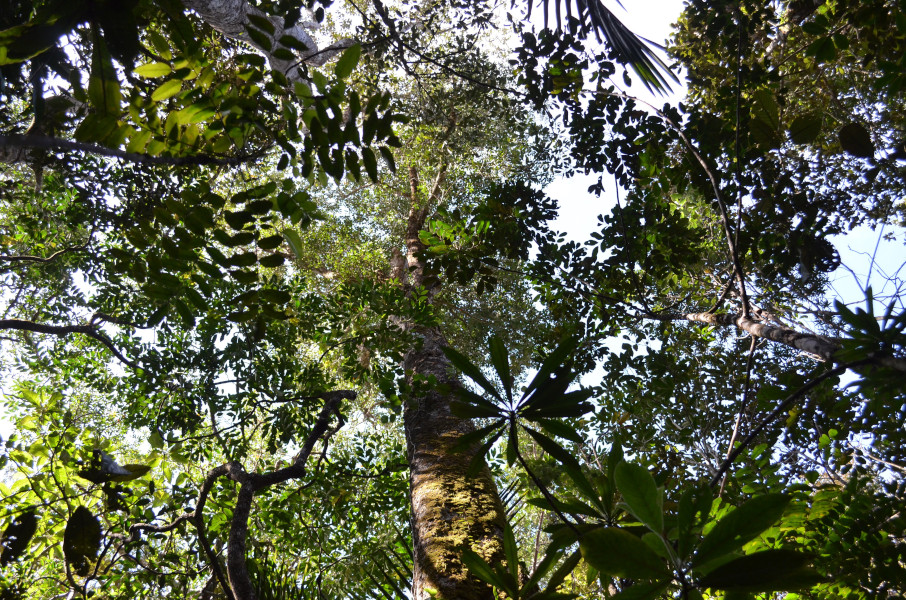
\includegraphics[keepaspectratio=true,
height=\paperheight]{figs/Canopy-NC} } \setbeamertemplate{navigation
symbols}{} \setbeamertemplate{blocks}[rounded][shadow=false]
\begin{frame}[plain] \vspace*{\stretch{100}} \begin{block}{} \begin{center}
\ldots~Gracias por su atención~\ldots \\ 
\url{https://ecology.ghislainv.fr/deforisk-qgis-plugin/es} \\ \textbf{>
Artículos > Referencias > Presentaciones} \\ 

\includegraphics[width=0.8\textwidth]{figs/partners_logos} \end{center}
\end{block} \end{frame} }
\end{document}
